
\section{Introducere}

% ============================================= Introducere =============================== ============================================= 
\subsection{Context }
    În aceasă lucrare este desrirsă implementare logicii de mișcare, în limbajul de planificare Planning Domain Definition Language (PDDL) a unui robot cu două brațe care se află într-un laborator de chimie și face diferite experimente cu substanțele pe care le are la dispoziție în laborator. Alegerea acestei teme de abordare este o pasiune veche pentru chimie. 
 \newline


\subsection{Descrierea acțiunilor pe care le face robotul chimist}
    
    Rolul robotului chimist este de a realiza diferite reacții chimice având la dispoziție mai multe substanțe (săruri, acizi și baze) precum și ustensile. Robotul are două brațe identificate prin brațul stâng și brațul drept. Pentru a realiza diferitele experimente chimice, el trebuie să măsoare cantitățile de substanțe reactante cu ajutorul paharelor berzelius și erlenmeyer, iar după măsurare va introduce reactantul într-o eprubetă. Reacția e finalizată în momentul în care în eprubetă se află două substanțe reactante. La final se va verifica rezultatul reacției \textbf{reactant1 +reactant2=result} astfel:
    \begin{itemize}
    \setlength\itemsep{0em}
        \item acid + bază = sare
        \item baza + sare = bază insolubilă
        \item acid + sare = precipitat 
    \end{itemize}
    Pentru realizarea măsurării, paharul berzelius sau erlenmeyer trebuie să fie curat înainte de a adăuga substanța pentru nu a apărea reacții nedorite cu cantitatea de substanță rămasă de la măsurătoarea anterioară. De aceea, roboțelul trebuie să spele recipientul dacă acesta nu e curat. De asemenea în timpul măsurării, robotul ține cu o mână paharul iar cu cealaltă va adăuga substanța de măsurat din recipientul ei (aici s-a considerat că trebuie doar să aibă acea mână liberă). \\ \newline
    Eprubeta trebuie să fie goală și curată înainte de a se ađăuga primul reactant. După adăugarea primului reactant se va aștepta adăugarea celui de-al doilea pentru realizarea reacției. În momentul în care în eprubetă sunt adăugate 2 reactanți aceasta se va considera plină și nu se vor mai adăuga alte substanțe.\\ \newline
    Recipientele și eprubeta pot fi puse pe stativ, iar de acolo robotelul chimist le poate lua cu brațele lui. Pentru măsurare, el trebuie să aibă în braț un recipient, iar celălalt să fie liber (pentru adăugarea substanței în recipient). Pentru curățarea recipientelor și a eprubetei ele tebuie ținute de un braț al robotului. În timpul acțiunii de adăugare a unui reactant din paharul de măsurat în eprubetă, într-unul din brațe robotul ține recipientul, iar in celălalt eprubeta. \\ \newline
    
    \begin{figure}[htp]
    \centering
    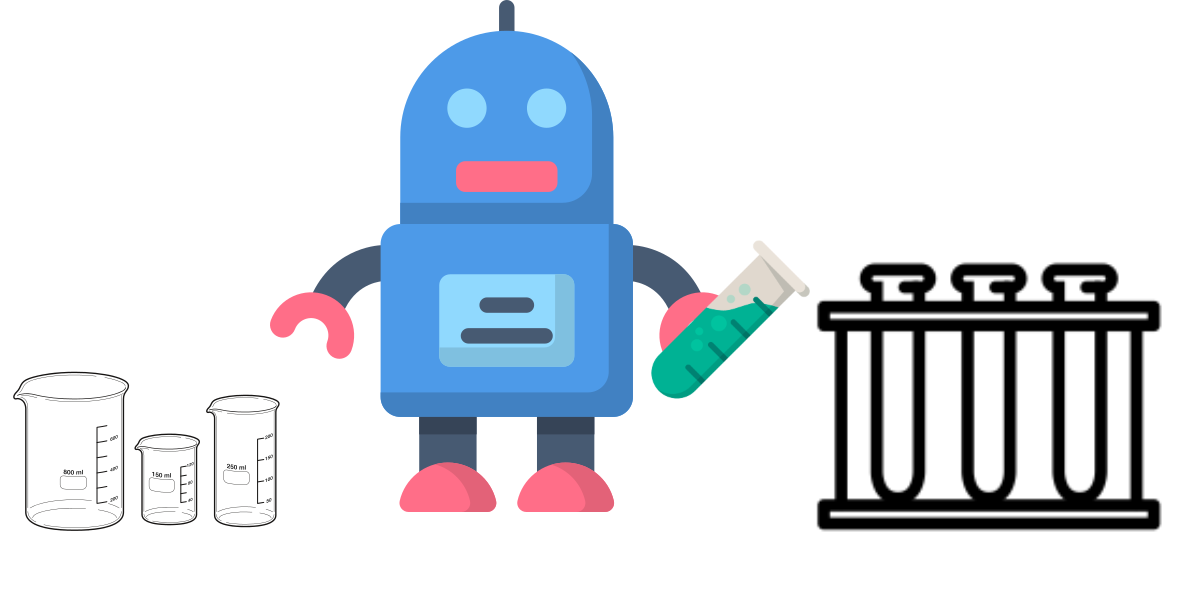
\includegraphics[width=10cm]{text/images/chemrob.png}
    \caption{Robotul chimist}
    \label{fig:galaxy}
\end{figure}


\section{PDDL Clasic}
\subsection{Definirea domeniului}
%-------------------------------------------------DOMENIU----------------------------------------------
\textbf{Code:}
% a se completa fisierul code/dfs.py
\inputminted[linenos]{python}{code/ClassicPDDL/robchemy.pddl}

\textbf{Explicații:}
\begin{itemize}
    \setlength\itemsep{0em}
    \item codul de mai sus descire domeniul cu tipurile și acțiunile pe care le poate executa robotul
    \item în secțiunea de \textbf{requirements} au fost setate pe lângă \textbf{strips} următoarele 
        \begin{itemize}
        \item typing : pentru ideea de moștenire; astfel că prin reactant ne vom referi fie la o sare, acid sau fi la o bază
        \item negative-preconditions : pentru folosirea negatiei în precondiții 
        \item adl : s-au folosit \textbf{forall} și \textbf{exists}; cu ajutorul acestora s-a verificat existența substanțelor în eprubete sau recipiente, astfel că în momentul în care se va 
        \item action-costs : acțiunile au costuri diferite
        \item   \begin{itemize}
                \setlength\itemsep{0em}
                \item cele mai costisitoare acțiuni vor fi cele de spălare a recipientelor de măsurat (3), iar apoi spălarea eprubetelor; Efectul costului se va observa în momentul în care robotul decide pentru măsurarea celui de-al doilea reactant să ia un al recipent de măsurat în loc să îl spele pe cel folosit pentru măsurarea primului reactant
                \end{itemize}
        \end{itemize}
    \item pentru definirea tipurilor s-a ținut seama de ideea de moștenire astfel 
        \begin{itemize}
        \item reactantul poate fi acid, baza sau sare
        \item bratul poate fi stang sau drept
        \item recipientele pot fi berzelius si erlenmeyer
        \end{itemize}
    \item pentru definrea predicatelor s-a ținut seama de toate posobilitătile în care se poate afla un recipient și eprubeta, dacă o substanță e într-un recipient sau eprubetă și de asemenea este descrisă și situația în care se pot afla brațele robotului (dacă acesta ține ceva în brațe sau nu)
    \item la linia 32 este definită funcția de cost ca număr; în cadrul definirii problemelor acest cost va trebui să fie inițializat
    \item actiunile gripp-recipient și drop-recipient se referă la ridicarea și lăsarea unui pahar de măsurat de către robot și au costul de 1
    \item acțiunea measure-reactant descrie condițiile ce trebuie îndeplinite pentru măsurarea cantității de reactant și efectele măsurării. Aceasta va aduce un cost de 2.
    \item first-reactant și second-reactant descriu introducerea reactanților în eprubeta; Eprubeta va fi plină după adăugarea celui de-al doilea reactant.
    \item clean-recipient si clean-eprubeta sunt acțiunile de curățare a recipientului și respectiv a eprubetei. Se observă folosirea sintaxei \textbf{forall} pentru a elimina și substanțele existente în recipient, respectiv eprubetă. Un recipient de măsurat trebuie să fie gol și curat pentru măsurarea substanțelor. Se ține cont de faptul că dacă paharul e gol, dar înainte a conținut o substanță.
    \item grip-eprubeta și drop-eprubeta vor descrie acțiunile de ridicare în braț a eprubetei de pe stativ și respectiv punerea acesteia înapoi pe stativ
    \item check-reactie-baza-acid, check-reactie-baza-sare și check-reactie-acid-sare sunt acțiunile care verifică rezultatul reacției din eprubetă. Se remarcă folosirea lui \textbf{exists} pentru verificarea existenței substanțelor reactante.
    
    

\end{itemize}
%------------------------------------------DEFINIREA PROBLEMEI----------------------------------
\vspace{0.75cm}
\subsubsection{Definirea problemei 1}
    În continuare e descrisă o problemă pentru robotul nostru. El trebuie să obțină în urma combinării reactantilor puși la dispozitie (o bază, o sare și un acid) un precipitat.  El are două recipiente curate pe stativ(masa): un pahar berzelius și unul erlenmeyer. Eprubeta în care se vrea să se facă reacția nu e curată și se află pe stativ. \\\newline
\textbf{Code:}
% a se completa fisierul code/bfs.py
\inputminted[linenos]{python}{code/ClassicPDDL/problemrob.pddl}


\textbf{Explicații:}
\begin{itemize}
    \setlength\itemsep{0em}
    \item sunt specificate condițiile atomice în secțiunea de init.
    \item la linia 34 se setează costul inițial la 0 și se dorește minimizarea acstuia. Cea mai concludentă actiune în obervarea cestei minimizări este decizia de a folosi pentru măsurarea substanțelor ambele pahare puse la dispoziție, in loc să folosească același pahar pa care să îl spele între măsurători (costul e mai ridicat pentru spălarea recipeientelor).
    \item pentru rezolvarea problemei, robotul trebuie să combine acid1 cu baza1 pentru a obtine un precipitat

\end{itemize}

\textbf{S-a folosit fast-downward pentru a afla planul de execuție a acțiunilor în îndeplinirea scopului. Pentru aceasta s-au folosit mai multe euristici de căutare și s-au comparat rezultatele }\\

\textbf{Comenzi:} \\
  \textcolor{red}{Cu euristica admisibila blind pentru astar:}
   \begin{itemize}
    \setlength\itemsep{0em}
    \item   fast-downward.py robchemy.pddl problemrob.pddl --heuristic "h=blind" --search "astar(h)"
    \item (gripp-recipient left1 berzelius1)\\
        (measure-reactant berzelius1 acid1 left1 right1)\\
       (gripp-eprubeta ep1 right1)\\
        (clean-eprubeta ep1 right1)\\
        (first-reactant berzelius1 acid1 left1 right1 ep1)\\
        (drop-recipient left1 berzelius1)\\
        (gripp-recipient left1 erlenmeyer1)\\
        (drop-eprubeta ep1 right1)\\
        (measure-reactant erlenmeyer1 sare1 left1 right1)\\
        (gripp-eprubeta ep1 right1)\\
        (second-reactant erlenmeyer1 sare1 left1 right1 ep1)\\
        (check-reactie-acid-sare ep1)\\
        ;cost = 15 (general cost)
    \item \textbf{S-au generat 14525 de stari; 4284 de stari au fost evaluate si au fost expandate 3228; costul e de 15 și este si cel minim deoarece cu euristica blind se obține un algortim de căutare asemănător cu ucs}
\end{itemize}

\textcolor{red}{Cu euristica hmax pentru astar:}
   \begin{itemize}
    \setlength\itemsep{0em}
    \item   fast-downward.py robchemy.pddl problemrob.pddl --heuristic "h=hmax" --search "astar(h)"
    \item gripp-recipient left1 berzelius1 (1)\\
measure-reactant berzelius1 acid1 left1 right1 (2)\\
gripp-eprubeta ep1 right1 (1)\\
clean-eprubeta ep1 right1 (2)\\
first-reactant berzelius1 acid1 left1 right1 ep1 (1)\\
drop-recipient left1 berzelius1 (1)\\
gripp-recipient left1 erlenmeyer1 (1)\\
drop-eprubeta ep1 right1 (1)\\
measure-reactant erlenmeyer1 sare1 left1 right1 (2)\\
gripp-eprubeta ep1 right1 (1)\\
second-reactant erlenmeyer1 sare1 left1 right1 ep1 (1)\\
check-reactie-acid-sare ep1 (1)\\
;cost = 15 (general cost)
    \item \textbf{S-au generat 2587 de stari; 995 de stari au fost evaluate si au fost expandate 548; Se observă că aplicarea acestei euristici aduce un număr mai mic de stări generate față de cazul anterior. De asemnea și numărul stărilor evaluate și expandate a scăzut considerabil. Costu e cel minim. Această euristică se bazează pe maximul dintre subcosturi. Lungimea planului a rămas tot de 12.  }
\end{itemize}


%-------------------------------------------------------------------------------------------------
 \textcolor{red}{Cu inconsistent and not admissible heuristic ff pentru astar:}
   \begin{itemize}
    \setlength\itemsep{0em}
    \item   fast-downward.py robchemy.pddl problemrob.pddl --heuristic "h=ff" --search "astar(h)"
    \item gripp-recipient left1 erlenmeyer1 (1) \\
measure-reactant erlenmeyer1 sare1 left1 right1 (2)\\
drop-recipient left1 erlenmeyer1 (1)\\
gripp-recipient left1 berzelius1 (1)\\
measure-reactant berzelius1 acid1 left1 right1 (2)\\
gripp-eprubeta ep1 right1 (1)\\
clean-eprubeta ep1 right1 (2)\\
first-reactant berzelius1 acid1 left1 right1 ep1 (1)\\
drop-recipient left1 berzelius1 (1)\\
gripp-recipient left1 erlenmeyer1 (1)\\
second-reactant erlenmeyer1 sare1 left1 right1 ep1 (1)\\
check-reactie-acid-sare ep1 (1)
    \item \textbf{S-au generat 134 de stari, un numar mult mai mic decât cifrele obținute la evaluările anterioare; acesta se datoreză faptului că problema s-a mai relaxat fiind aplicată o euristică care nu e admisibilă; 87 de stari au fost evaluate si au fost expandate 26; În ceea ce priveste costul si numarul de pasi nu au apărut modificări. costul e de 15; 12 pasi}
\end{itemize}

\textcolor{red}{Cu inconsistent and not admissible heuristic cg pentru astar:}
   \begin{itemize}
    \setlength\itemsep{0em}
    \item   fast-downward.py robchemy.pddl problemrob.pddl --heuristic "h=cg" --search "astar(h)"
    \item gripp-recipient left1 berzelius1 (1) \\
measure-reactant berzelius1 acid1 left1 right1 (2)\\
gripp-eprubeta ep1 right1 (1)\\
drop-recipient left1 berzelius1 (1)\\
gripp-recipient left1 erlenmeyer1 (1)\\
drop-eprubeta ep1 right1 (1)\\
measure-reactant erlenmeyer1 sare1 left1 right1 (2)\\
gripp-eprubeta ep1 right1 (1)\\
clean-eprubeta ep1 right1 (2)\\
first-reactant erlenmeyer1 sare1 left1 right1 ep1 (1)\\
drop-recipient left1 erlenmeyer1 (1)\\
gripp-recipient left1 berzelius1 (1)\\
second-reactant berzelius1 acid1 left1 right1 ep1 (1)\\
check-reactie-acid-sare ep1 (1)\\
    \item \textbf{S-au generat 317 de stari, problema de căutare s-a mai relaxat fiind aplicată o euristică care nu e admisibilă; 211 de stari au fost evaluate si au fost expandate 67. Aceste valori sunt mult mai mici față de ce am obținut pentru blind și hmax, dar observăm că nu am obtinut valori mai bune față de evaluarea cu euristica "ff" ; Numărul de pași/ lungimea planului a crescut, din cazua faptului că se folosește o eruistică ce nu e admisibilă, acesta a urcat la 14. Nici costul nu mai e cel minim, ci s-a ajuns o valoare de 17.}
\end{itemize}

\textcolor{red}{Cu inconsistent and not admissible heuristic ff pentru wighted astar (2):}
   \begin{itemize}
    \setlength\itemsep{0em}
    \item   fast-downward.py robchemy.pddl problemrob.pddl --heuristic "h=ff" --search "astar(weight(h,2))"
    \item gripp-recipient left1 erlenmeyer1 (1)\\
measure-reactant erlenmeyer1 sare1 left1 right1 (2)\\
drop-recipient left1 erlenmeyer1 (1)\\
gripp-recipient left1 berzelius1 (1)\\
measure-reactant berzelius1 acid1 left1 right1 (2)\\
gripp-eprubeta ep1 right1 (1)\\
clean-eprubeta ep1 right1 (2)\\
first-reactant berzelius1 acid1 left1 right1 ep1 (1)\\
drop-recipient left1 berzelius1 (1)\\
gripp-recipient left1 erlenmeyer1 (1)\\
second-reactant erlenmeyer1 sare1 left1 right1 ep1 (1)\\
check-reactie-acid-sare ep1 (1)\\
; cost = 15 (general cost)
    \item \textbf{Rezultatele obținute în urma acestei evaluări sunt foarte bune. Costul obținut e cel minim (15), iar numărul de pași este 12. Au fost generate 118 stari, un număr foarte bun. 83 de stari au fost evaluate si au fost expandate 22; Aceste rezultate sunt foarte bune având in vedere problema de căutare.}
    \item Observam scaderea numarlui de stari expandate fata de celelalte
\end{itemize}


\textcolor{red}{Cu cu greedy si ff euristica:}
   \begin{itemize}
    \setlength\itemsep{0em}
    \item   fast-downward.py robchemy.pddl problemrob.pddl --search "eager\_greedy([ff])"
    \item gripp-recipient left1 erlenmeyer1 (1)\\
measure-reactant erlenmeyer1 sare1 left1 right1 (2)\\
drop-recipient left1 erlenmeyer1 (1)\\
gripp-recipient left1 berzelius1 (1)\\
measure-reactant berzelius1 acid1 left1 right1 (2)\\
gripp-eprubeta ep1 right1 (1)\\
clean-eprubeta ep1 right1 (2)\\
first-reactant berzelius1 acid1 left1 right1 ep1 (1)\\
drop-recipient left1 berzelius1 (1)\\
gripp-recipient left1 erlenmeyer1 (1)\\
second-reactant erlenmeyer1 sare1 left1 right1 ep1 (1)\\
check-reactie-acid-sare ep1 (1)\\
; cost = 15 (general cost)
    \item \textbf{Au fost generate 118 stari. 83 de stari au fost evaluate si au fost expandate 22; costul e de 15; 12 pasi}
    \item \textbf{Comparativ cu aplicarea euristicii ff pe astar, rezultetele obținute pentru greedy sunt puțin mai bune. Diferența nu e majoră, dar pentru probleme de căutare mai complexe se va simți această difereță;}
\end{itemize}
%---------------------------------------------------------------------------------------------
\textcolor{red}{Cu cu greedy si cg euristica:}
   \begin{itemize}
    \setlength\itemsep{0em}
    \item   fast-downward.py robchemy.pddl problemrob.pddl --search "eager\_greedy([cg])"
    \item 
gripp-recipient left1 berzelius1 (1)\\
measure-reactant berzelius1 acid1 left1 right1 (2)\\
gripp-eprubeta ep1 right1 (1)\\
drop-recipient left1 berzelius1 (1)\\
gripp-recipient left1 erlenmeyer1 (1)\\
drop-eprubeta ep1 right1 (1)\\
measure-reactant erlenmeyer1 sare1 left1 right1 (2)\\
gripp-eprubeta ep1 right1 (1)\\
clean-eprubeta ep1 right1 (2)\\
first-reactant erlenmeyer1 sare1 left1 right1 ep1 (1)\\
drop-recipient left1 erlenmeyer1 (1)\\
gripp-recipient left1 berzelius1 (1)\\
second-reactant berzelius1 acid1 left1 right1 ep1 (1)\\
check-reactie-acid-sare ep1 (1)
    \item \textbf{Numărul de stări generate este de 131. 94 de stari au fost evaluate si au fost expandate 28; costul e de 17; 14 pasi}
    \item Față de aplicarea euristicii cg pe algorimtul astar, observăm cărezultatele pentru greedy în ceea ce privește numărul de stări generate și evaluatre e mai mic. În schimb, costul e mai mare și la fel numărul de pași.  
\end{itemize}
\vspace{1.75cm}


%----------------------------------PROBLEMA 2---------------------------------------------------
\subsubsection{Definirea problemei 2}
   La problema 1 s-a adaugat sa se obtina si o sare in eprubeta 2\\\newline
\textbf{Code:}
% a se completa fisierul code/bfs.py
\inputminted[linenos]{python}{code/ClassicPDDL/problemrob2.pddl}
Solutia la problema 2 cu euristica ff la algoritmul de căutare astar weighted: \\
fast-downward.py robchemy.pddl problemrob2.pddl --heuristic "h=ff" --search "astar(weight(h,2))" \\
gripp-recipient left1 erlenmeyer1 (1)\\
measure-reactant erlenmeyer1 sare1 left1 right1 (2)\\
gripp-eprubeta ep1 right1 (1)\\
clean-eprubeta ep1 right1 (2)\\
first-reactant erlenmeyer1 sare1 left1 right1 ep1 (1)\\
clean-recipient erlenmeyer1 left1 (3)\\
drop-eprubeta ep1 right1 (1)\\
measure-reactant erlenmeyer1 acid1 left1 right1 (2)\\
drop-recipient left1 erlenmeyer1 (1)\\
gripp-recipient left1 berzelius1 (1)\\
measure-reactant berzelius1 baza1 left1 right1 (2)\\
gripp-eprubeta ep2 right1 (1)\\
first-reactant berzelius1 baza1 left1 right1 ep2 (1)\\
drop-eprubeta ep2 right1 (1)\\
clean-recipient berzelius1 left1 (3)\\
measure-reactant berzelius1 acid1 left1 right1 (2)\\
gripp-eprubeta ep1 right1 (1)\\
second-reactant berzelius1 acid1 left1 right1 ep1 (1)\\
drop-recipient left1 berzelius1 (1)\\
gripp-recipient left1 erlenmeyer1 (1)\\
drop-eprubeta ep1 right1 (1)\\
gripp-eprubeta ep2 right1 (1)\\
second-reactant erlenmeyer1 acid1 left1 right1 ep2 (1)\\
check-reactie-acid-sare ep1 (1)\\
check-reactie-baza-acid ep2 (1)\\
; cost = 34 (general cost)\\
\textbf{Statistici: } 
Lungimea planului: 25 pași
Cost : 34
Stari generate: 1836
Stari expandate: 387
Stari evaluate: 894

Se observă o creștere a numărului de stări expandate cu mărirea problemei de căutare, dar rezultatele sunt tot mici față de rezultatele pe care le-am întâmpinat în cadrul unei probleme mai mici, dar cu căutarea pe o euristică slabă.


\vspace{0.75cm}
%-------------------------------------------CONFORMANT----------------------------------------------
\section{Conformant}
Au fost necesare mici modificări pentru a trece domeniul definit în cadrul planificării clasice complet observabile, într-un mediu parțial observabil. Am fost nevoit să scot costurile și de asemnea o verificare cu exists în precondiția unei acțiuni pentru că se genera eroarea legată de faptul că nu se suportă disjuncțiile. În continuare se regăsește codul pentru domeniu.

\subsection{Definirea domeniului}
\textbf{Code:}
% a se completa fisierul code/dfs.py
\inputminted[linenos]{python}{code/Conformant/robchemy.pddl}
\textbf{Explicații:}
\begin{itemize}
    \setlength\itemsep{0em}
    \item modificările aduse domeniului se pot observa în definirea acțiunilor \textit{first-reactant} și \textit{second-reactant}. S-au scos precondițiile ca recipientul să conțină o substanța și s-au pus la effect cu \textbf{when} in cazul în care există substanța trimisă ca parametru în recipientul de măsurat, să se adauge în eprubetă.

\end{itemize}

%-------------------------------------definirea problemei pentru conformant--------------------------
\subsection{Definirea problemei}
În cadrul problemei s-au adăugat situatii incerte/necunoscute prin UNKNOWN.
\textbf{Code:}
% a se completa fisierul code/dfs.py
\inputminted[linenos]{python}{code/Conformant/problemrob.pddl}
\textbf{Explicații:}
\begin{itemize}
    \setlength\itemsep{0em}
    \item starea inițială se definește ca fiind necunoscută. Stiim că cele două pahare sunt pline cu un acid1 sau baza1 și nu se știe exact ce substanță se află. Fie acid1 se află în paharul berzelius, iar baza1 în paharul erlenmeyer, fie acid1 se află în pahareul erlenmeyer, iar baza1 se află în paharul berzelius.
    \item Rezultatul obținut prin apelul : \textit{./Conformant-ff -o robchemy.pddl -f problemrob.pddl}\\
    \begin{itemize}
    \setlength\itemsep{0em}
        \item 0: GRIPP-RECIPIENT RIGHT1 BERZELIUS1 
        \item 1: CLEAN-RECIPIENT BERZELIUS1 RIGHT1
        \item 2: MEASURE-REACTANT BERZELIUS1 ACID1 RIGHT1 LEFT1 
        \item 3: GRIPP-EPRUBETA EP1 LEFT1
        \item 4: FIRST-REACTANT BERZELIUS1 ACID1 RIGHT1 LEFT1 EP1
        \item 5: CLEAN-RECIPIENT BERZELIUS1 RIGHT1
        \item 6: DROP-EPRUBETA EP1 LEFT1
        \item 7: MEASURE-REACTANT BERZELIUS1 BAZA1 RIGHT1 LEFT1
        \item 8: GRIPP-EPRUBETA EP1 LEFT1
        \item 9: SECOND-REACTANT BERZELIUS1 BAZA1 RIGHT1 LEFT1 EP1
        \item 10: CHECK-REACTIE-BAZA-ACID EP1
     \end{itemize}
     \item Cea mai simplă soluție pe care o va aborda roboțelul e de a spăla recipientul, deoarece nu cunoaște exact ce substanță se află în recipienete. Mă așteptam să introducă ambele substanțe din recipiente fiindcă se ajungea la rezultat, doar el a ales să spele recipientele și să adauge apoi reactanții necesari pentru obtinerea sării.
     \item Cu hill-climbing nu s-a putut rezolva problema și s-a continuat cu Best-first Search
     \item s-au realizat 159 de state transition bazate pe CNF
     \item 
     \end{itemize}
    
%-------------------------------------------CONTINGENT------------------------------------------------
\section{Contingent}
Au fost necesare mici modificări pentru a trece domeniul definit în cadrul planificării clasice complet observabile, într-un mediu parțial observabil. Am fost nevoit să scot costurile și de asemnea o verificare cu exists în precondiția unei acțiuni pentru că se genera eroarea legată de faptul că nu se suportă disjuncțiile. În continuare se regăsește codul pentru domeniu. S-a renunțat la when-urile din cadrul acțiunilor \textit{first-reactant} și \textit{second-reactant} și s-a revenit la adăugarea condiției în precondiții (față de codul pentru conformant). De asemenea s-a adăugat un observator. 

\subsection{Definirea domeniului}
\textbf{Code:}
% a se completa fisierul code/dfs.py
\inputminted[linenos]{python}{code/Contingent/robchemy.pddl}

\textbf{Explicații:}
\begin{itemize}
    \setlength\itemsep{0em}
    \item ceea ce este de specificat este adăugarea observatorului \textbf{senseContain}; Prin adăugarea acestui observator, roboțelul poate observa ce substanțe se află în recipiente. În acest caz, el poate să decidă dacă se poate folosi de ce are deja în recipiente pentru a-și îndeplini scopul.   

\end{itemize}

\subsection{Definirea problemei}
În cadrul problemei s-au adăugat situații incerte/necunoscute prin UNKNOWN. La fel ca și la conformant avem același scop.\\ \\
\textbf{Code:}
% a se completa fisierul code/dfs.py
\inputminted[linenos]{python}{code/Contingent/problemrob.pddl}
\textbf{Explicații:}
\begin{itemize}
    \setlength\itemsep{0em}
    \item starea inițială se definește ca fiind necunoscută. Este la fel ca la conformant. Știim că cele două pahare sunt pline cu un acid1 sau baza1 și nu se știe exact ce substanță se află. Fie acid1 se află în paharul berzelius, iar baza1 în paharul erlenmeyer, fie acid1 se află în pahareul erlenmeyer, iar baza1 se află în paharul berzelius.
    \item Rezultatul obținut prin apelul : \textit{./Contingent-ff -o robchemy.pddl -f problemrob.pddl}\\
\end{itemize}
\textbf{Rezultate}\\
-------------------------------------------------\\
  0||0 --- GRIPP-EPRUBETA EP1 LEFT1 --- SON: 1||0\\
-------------------------------------------------\\
  1||0 --- SENSECONTAIN BAZA1 ERLENMEYER1 --- TRUESON: 2||0 --- FALSESON: 2||1\\
-------------------------------------------------\\
  2||0 --- GRIPP-RECIPIENT RIGHT1 BERZELIUS1 --- SON: 3||0\\
  2||1 --- GRIPP-RECIPIENT RIGHT1 BERZELIUS1 --- SON: 3||1\\
-------------------------------------------------\\
  3||0 --- FIRST-REACTANT BERZELIUS1 ACID1 RIGHT1 LEFT1 EP1 --- SON: 4||0\\
  3||1 --- FIRST-REACTANT BERZELIUS1 BAZA1 RIGHT1 LEFT1 EP1 --- SON: 4||1\\
-------------------------------------------------\\
  4||0 --- DROP-RECIPIENT RIGHT1 BERZELIUS1 --- SON: 5||0\\
  4||1 --- DROP-RECIPIENT RIGHT1 BERZELIUS1 --- SON: 5||1\\
-------------------------------------------------\\
  5||0 --- GRIPP-RECIPIENT RIGHT1 ERLENMEYER1 --- SON: 6||0\\
  5||1 --- GRIPP-RECIPIENT RIGHT1 ERLENMEYER1 --- SON: 6||1\\
-------------------------------------------------\\
  6||0 --- SECOND-REACTANT ERLENMEYER1 BAZA1 RIGHT1 LEFT1 EP1 --- SON: 7||0\\
  6||1 --- SECOND-REACTANT ERLENMEYER1 ACID1 RIGHT1 LEFT1 EP1 --- SON: 7||1\\
-------------------------------------------------\\
  7||0 --- CHECK-REACTIE-BAZA-ACID EP1 --- SON: 8||-1\\
  7||1 --- CHECK-REACTIE-BAZA-ACID EP1 --- SON: 8||-1\\
-------------------------------------------------\\
tree layers: 8\\
total nr. actions: 14\\
\begin{itemize}
    \setlength\itemsep{0em}
    \item se observă că roboțelul primește o informație de la senzori; Aici problema se va ramifica în două în funcție de ce conține în paharul erlenmeyer; Dacă în erlenmeyer se găsește baza1, atunci se va merge pe ramura 0, iar în caz contrar se va continua pe ramura 1 (în care acid1 se va afla în paharul erlenmeyer).
    \item arborele format va avea 8 nivele, iar numărul total de acțiuni va fi de 14. 
    \item mai jos se regăsește arborele de planificare în funcție de decizia pe care o să o ia roboțelul aflând infomrația că are substanțele necesare obținerii sării în cele două recipiente, scutindu-l astfel de a măsura cantitatea de substanțe.

   \item
\begin{figure}[htp]
    \centering
    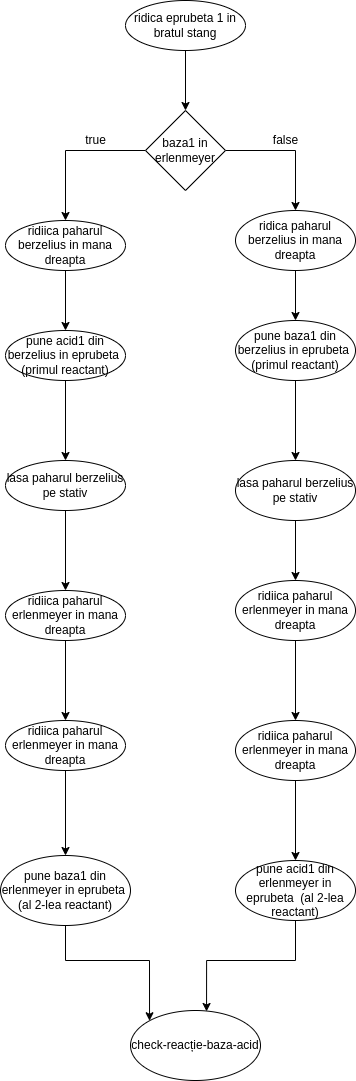
\includegraphics[width=10cm,height=20cm]{text/images/arbore.png}
    \caption{Arbore}
    \label{fig:galaxy}
\end{figure}
\end{itemize}














\subsection{References}
R. Stuart, N. Peter, Artificial Intelligence: A Modern Approach, 4th US ed., capitol 3, [online]